\documentclass[a4paper,12pt,titlepage,oneside]{article}

\usepackage[italian]{babel}
\usepackage[utf8]{inputenc}
\usepackage{listings} 
\usepackage{cite}
\lstset{
    literate={~} {$\sim$}{1}
}
\usepackage{amsmath,amssymb,amsfonts,amsthm,graphicx,mathrsfs,braket}
\usepackage{hyperref}
\usepackage{times}
\usepackage[left=2.5cm, right=2.5cm]{geometry}
\usepackage{parskip}
\usepackage{xcolor}
\usepackage{algorithm}
\usepackage[noend]{algpseudocode}
\makeatletter
\def\BState{\State\hskip-\ALG@thistlm}
\makeatother
\hypersetup{colorlinks=false,
allbordercolors=white}
\setcounter{secnumdepth}{4} 
\setcounter{tocdepth}{3}
\linespread{1.5}
\begin{document}
\newcommand\tab[1][1cm]{\hspace*{#1}}
\thispagestyle{empty}
\begin{figure}
	\centering
	\vspace*{-2cm}	
	
\includegraphics[scale=0.4]{logo.png}
	\label{fig:logo}
\end{figure}
\centerline{{\LARGE UNIVERSIT\`{A} DEGLI STUDI DI CATANIA}}
\centerline{DIPARTIMENTO DI MATEMATICA E INFORMATICA} \centerline{CORSO DI LAUREA MAGISTRALE IN INFORMATICA}
\centerline{\rule{16cm}{0.2mm}}\vspace*{2cm}
\centerline{\huge{UNCAPACITATED FACILITY LOCATION PROBLEM}}
\centerline{\huge{}}
\centerline{\huge{WITH}}
\centerline{\huge{}}
\centerline{\huge{IMMUNOLOGICAL ALGORITHM}}
\vspace*{2cm}
\centerline{\rule{5cm}{0.2mm}}\medskip
\centerline{\Large{PROGETTO DI COMPUTAZIONE NATURALE}}
\centerline{\rule{5cm}{0.2mm}}
\vspace*{4cm}

\centerline{\Large{Andrea Sequenzia}}
\centerline{\Large{Matricola: W82000160}}


\vspace*{2cm}

%\vspace{1cm}
\enlargethispage{10cm}
\centerline{\rule{16cm}{0.2mm}} 
\centerline{ANNO ACCADEMICO 2018/2019} 
\newpage
\tableofcontents
\newpage

\section{Introduzione}

\section{Definizione del problema}

In un problema UFLP, ci sono $m$ clienti da servire ed $n$ possibili location dove poter stabilire delle facilities che servano i clienti e soddisfare la domanda. Ogni facility $i$ ha un costo fisso di installazione $f_{i}$. Un costo di trasporto $c_{ij}$ per servire il il cliente $j$ dalla facility $i$. Le facility non hanno limiti nelle capacità di quanto possono servire e non ci devono essere clienti non soddisfatti. L'obiettivo finale è quello di stabilire quali facility attivare, soddisfando tutti i clienti, minimizzando il costo per ottenere ciò. Formalmente:

\begin{equation*}
\begin{aligned}
& \underset{}{\text{minimize}}
& & \sum_{i=1}^{n} \sum_{j=1}^{m}c_{ij}x_{ij} + \sum_{i=1}^{n}f_{i}y_{i} \\
& \text{subject to}
& & \sum_{i=1}^{n}x_{ij}=1, \quad j=1,...,m, \\
& & & x_{ij}\leq y_{i}, \quad i=1,...,n, j=1,...,m,\\
& & &  x_{ij},y_i=0,1,\quad i=1,...,n, j=1,...,m
\end{aligned}
\end{equation*}
dove \\
$c_{ij} =$ il costo per soddisfare la domanda del cliente $j$ dalla facility $i$; \\
$f_{i} =$ il costo per stabilire la facility nella location $i$ \\

$x_{ij}=\left\{\begin{aligned}
 & 1 \quad \text{se il cliente j viene servito dalla facility i},\\ 
 & 0 \quad altrimenti;
\end{aligned}\right.$

$y_{i}=\left\{\begin{aligned}
 & 1 \quad \text{se la facility è stabilita nella location i},\\ 
 & 0 \quad altrimenti;
\end{aligned}\right.$

\begin{figure}
  \centering
  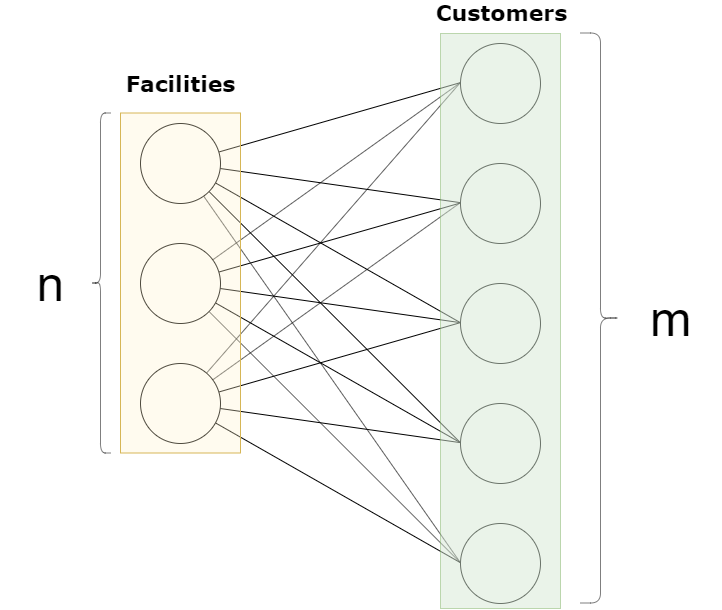
\includegraphics[scale=.3]{UFLP_Sample.png}
  \caption{Esempio problema UFLP}
\end{figure}

Il problema può essere matematicamente decomposto in due sottoproblemi indipendenti \cite{Sultan1999}:
\begin{enumerate}
\item \textbf{Location}, ovvero le facilities da stabile ($y_{i}$)
\item \textbf{Allocation}, per le facility stabilite, determinare la distribuzione e quindi quali archi usare per ogni customer ($x_{ij}$) 
\end{enumerate}

Per ogni soluzione del problema di Location, una soluzione ottima può essere ottenuta per il problema Allocation. Dato un vettore $y$, può essere ottenuto un assegnamento ottimale delle $x_{ij}$ usando la seguente formula:

\begin{equation*}
\begin{aligned}
& k:\min_{k}c_{kj}, \quad k = 1,...,n \\
& x_{ij}=\left\{\begin{aligned}
& 1 \quad \text{se i=k},\\ 
& 0 \quad altrimenti;
\end{aligned}\right.
\end{aligned}
\end{equation*}

Quindi il problema si riduce a determinare l'assegnamento di facilities ottimale.
\section{Algoritmo immunologico}

Un algoritmo immunologico è un algoritmo basato sul clonal selection principle, esso è un ottimo esempio di strategia intelligente in cui l'adattamento opera a livello locale, mentre un comportamento complesso agisce a livello globale. L'idea di questa tipologia di algoritmo deriva dal sistema immunitario naturale, in particolare da come le cellule si adattano per legarsi ed eliminare
entità straniere, meglio conosciute come Antigene. Questo algoritmo è basato su due entità: gli \textbf{antigeni} che rappresentano il problema da affrontare e le \textbf{B cell} (Linfocita B) che rappresentano un punto nello spazio di ricerca \cite{Pavone}. L'algoritmo crea una popolazione di B cell, esse cresceranno e si perfezioneranno nel corso di un numero prefissato di generazioni, morendo quando hanno raggiunto un'età prefissata. La qualità delle B cell si valuta attraverso una funzione di fitness. Come primo passo, l'algoritmo genera una popolazione random $P^{(t)}$ e successivamente usa i seguenti operatori in sequenza:
\begin{enumerate}
\item \textbf{Cloning}: questo operatore simula il meccanismo di proliferazione di un sistema immunitario. Esso genera una popolazione intermedia $P^{(clo)}$ copiando \textit{dup} volte ogni B cell, assegnando un'età casuale tra $[0, \frac{2}{3} \tau_{b}]$, la nuova popolazione così fatta sarà delle dimensioni \textit{$d \times dup$}. 
\item \textbf{Inversely Hypermutation}: il compito di questo operatore è quello di esplorare il vicinato di ogni clone creato dal precedente operatore. Ciò viene compiuto eseguendo $M$ mutazioni ad ogni elemento di $P^{(clo)}$ e ottenendo la nuova popolazione $P^{(hyp)}$. Per determinare $M$, viene adottata una legge inversamente proporzionale al valore della fitness: più piccolo (minimizzazione) è il valore valore della funzione di fitness, meno mutazioni saranno fatte alla B cell. Dato un clone $x$, per determinare il valore $M$ è necessaria la seguente formula:
\begin{equation}
\alpha=e^{-\rho\hat{f}(x)}
\end{equation}
dove $\alpha$ rappresenta il mutation rate,$\rho$ lo shape del mutation rate e $\hat{f}(x)$ è il valore della funzione di fitness normalizzato tra $[0,1]$. Il numero di mutazioni $M$ è dato da:
\begin{equation}
M = \lfloor(\alpha \times l) + 1 \rfloor
\end{equation}
dove $l$ è la lunghezza di una B cell. 
\item \textbf{Aging}: questo operatore aiuta l'algoritmo a saltare via dagli ottimi locali. Per ottenere ciò, rimuove le vecchie B cell dalla popolazione iniziale e da quella ipermutata. L'eliminazione avviene quando l'età (che viene incrementata ad ogni fine generazione) raggiunge l'età massima ($\tau_{B}$). Così facendo, si produce alta diversità e si aiuta l'algoritmo ad evitare le convergenze premature. Viene anche fatta un eccezione nella rimozione, ovvero lasciare la migliore soluzione nella popolazione anche se ha raggiunto la massima età. Questa variante viene chiamata \textit{elitist aging operator}.
\item \textbf{($\mathbf{\mu + \lambda}$)-Selection}: l'ultimo operatore sceglie le migliori \textit{d} B cell da mandare alla generazione successiva. In questo caso si ha $\mu = d$ e $\lambda = (d \times dup)$, questo operatore riduce la grandezza della popolazione di grandezza $\lambda \geq  \mu$ in nuova popolazione di dimensione $\mu=d$. A volte può accadere che siano sopravvissuti meno B cell di quelli richiesti per avere la giusta dimensione della popolazione. In questo caso, vengono generate casualmente delle nuove B cell per raggiungere la giusta dimensione.
\begin{algorithm}
\caption{Immunological Algorithm (d, dup, $\rho$, $\tau_{B}, n\_gen$)}\label{euclid}
\begin{algorithmic}[1]
\State $t \gets 0$
\State $P^{(t)} \gets Initialize\_Population(d)$;
\State $Compute\_Fitness(P^{(t)})$;
\Repeat
\State $P^{(clo)} \gets Cloning(P^{(t)},dup)$;
\State $P^{(hyp)} \gets Hypermutation(P^{(clo)},\rho)$;
\State $Compute\_Fitness(P^{(hyp)})$
\State $(P_{a}^{(t)},P_{a}^{(hyp)}) \gets Aging(P^{(t)}, P^{(hyp)}, \tau_B)$
\State $P^{(select)} \gets (\mu + \lambda)-Selection(P_a^{(t)}, P_a^{(hyp)})$;
\State $Compute\_Fitness(P^{(t+1)})$;
\State $t \gets t + 1$;
\Until number of generation reached
\end{algorithmic}
\end{algorithm}
\end{enumerate}

\section{Implementazione}
Per implementare questo algoritmo immunologico e adattarlo al problema UFLP è stato usato il linguaggio di programmazione di Python e per le operazioni sui grafi, è stata usata la libreria \textbf{networkx}\footnote[10]{https://networkx.github.io/}. Per rappresentare ogni soluzione (B cell) sono stati usati dei vettori binari, dove 0 indica che la facility è disattivata e 1 la facility è attivata. La funzione di fitness viene calcolata tenendo conto della configurazione del vettore delle facilities, per ogni customer viene considerato l'arco (disponibile) con il minore costo così da soddisfare i requisiti del sottoproblema Allocation. Gli script creati sono i seguenti:
\begin{itemize}
  \item \textbf{immune\_algorithm.py}: tramite questo script viene eseguito tutto il flusso dell'algoritmo, quindi vengono implementati i vari operatori e gestita la popolazione;
  \item \textbf{instance\_generator.py}: questo script genera un'istanza dal problema da un file di testo che segue un determinato formato dati;
  \item \textbf{solution.py}: questa classe implementa una B cell, in essa è contenuta una permutazione (vettore binario), l'età, la fitness e il metodo per calcolarla. Inoltre è implementato il metodo per eseguire l'ipermutazione;
  \item \textbf{main.py}: questo è lo script da eseguire per eseguire l'intero programma, da esso si possono settare i vari parametri: numero delle generazioni da eseguire, numero di B cell della popolazione, numero di clonazioni, il parametro $\rho$ per l'hypermutation e $\tau_{B}$;
\end{itemize}
\section{Esperimenti}

\section{Conclusioni}
\newpage
\bibliography{bibliografia}{}
\bibliographystyle{plain}
\end{document}
